\documentclass{article}
\usepackage[utf8]{inputenc}
\usepackage[english, science, small]{ku-frontpage}
\usepackage{tabularx}
\usepackage{indentfirst}

\title{Software Engineering}
\subtitle{First hand-in}
\author{Matias Korn(crd551), Samuel Korn(rxq534), Nikolin Prenga (hpq143), Silvan Adrian (zlp432)}
\date{\today}

\begin{document}

\maketitle

\section{Solution and problem domain}
Citizens have the possibility to apply for loss of earnings. Loss of earnings means, that the earnings the citizen has missed out on, due to being occupied of taking care of a child. There are many actors involved when the citizen apply for loss of earnings. First off, there is the case-worker, who receives the application from the citizen. The case-worker is working at a municipality council. The municipality council has to comply with the law and paragraph 42 and the rules that are provided from the ministry of social affairs.

\vspace{2mm}

The ministry of social affairs lay down the rules of:
(1) How big a possible cap of allowed compensation is.
(2) How much the pension scheme is obligated to contribute with. (3) How the calculation of the actual compensation is made. (4) What the limit is of how much the pension scheme is obligated to contribute with. (5) How much of the loss on the pension contribution shall be paid by the receiver and municipal council.

\vspace{2mm}

As mentioned, the case-workers handles the cases and receives all the necessary information, for complying with paragraph 42. First of, the case-worker has to establish, if there are grounds for compensation. (1) The child has to be under 18. (2) The conditions on the child's health have to abide by the law, for that the child's health record has to be collected from the health care system. The health record has to confirm, that it is most expedient for the mother or father to the care of the child, at home or has been placed in care under section 52(3)(vii). If that is the case, the condition is, that it is most expedient for a parent to be there. It might be difficult to establish, if that is the case, based on the health record, if it is not explicitly stated, therefore it might be necessary to collect a confirmation by the child's doctor. (3) Loss of income has to be established, for that the necessary bank statements have to be provided.

\vspace{2mm}

Our solution is concerned with case management. We have to provide a platform for collecting, recording the progress and the final decisions that have been made and what grounds there has been for them. The following actors are directly involved in our system: (1) the citizen, (2) the case-worker, (3) the minister of social affairs(external system), (4) the law that decides if the citizen is permitted for loss of earnings, (5) the payment system(external system), that is available for the municipal council. Our solution will handle the information gathering and storing. It resolves applications by an unbiased majority vote and calculates the compensation amount based on the numbers provided by the minister of social affairs.

\section{Scenarios}

\subsection*{Application approved}

Alice, a parent, has a child with a serious chronic illness. She logs into the OCM system as a citizen, fills out a form, attaches any relevant documentation and submits the application. There does not exist any prior applications from Alice, so the system annotates it as a new case.

\vspace{2mm}

The system assigns the application to caseworker Bob. He logs into the system as a caseworker. He picks Alice's application from an overview of assigned cases. He validates documentation authenticity and data entered in form by Alice. He approves and submits the application.

\vspace{2mm}

The system assigns the application to another caseworker Charles. He processes the application in the same manner as Bob and submits it once it is approved.

\vspace{2mm}

With approvals from two random caseworkers, the system annotate the case as approved and calculates the compensation based on the data contained in the application. The system sends a response to Alice's e-mail that her application was approved, including the details regarding her compensation. The system archives the case.

\subsection*{Application rejected}

Alice, a parent, has a child with a fever. She logs into the OCM system as a citizen, fills out a form, attaches any relevant documentation and submits the application. There does not exist any prior applications from Alice, so the system annotates it as a new case.

\vspace{2mm}

The system assigns the application to caseworker Bob. He logs into the system as a caseworker. He picks Alice's application from an overview of assigned cases. He validates documentation authenticity. The applicant is not eligible for compensation, so he rejects and submits the application.

\vspace{2mm}

The system assigns the application to another caseworker Charles. He concludes the same as Bob. Charles also rejects and submits the application.

\vspace{2mm}

With rejections from two random caseworkers, the system annotate the case as rejected. The system sends a response to Alice's e-mail that her application was rejected. The system archives the case.

\subsection*{Disputed application approval}

Alice, a parent, has a child with an ambiguous illness in the context of "loss of earnings" legislation. She logs into the OCM system as a citizen, fills out a form, attaches any relevant documentation and submits the application. There does not exist any prior applications from Alice, so the system annotates it as a new case.

\vspace{2mm}

The system assigns the application to caseworker Bob. He logs into the system as a caseworker. He picks Alice's application from an overview of assigned cases. He validates documentation authenticity and data entered in form by Alice. He approves and submits the application.

\vspace{2mm}

The system assigns the application to another caseworker Charles. He validates documentation authenticity and data entered in form by Alice. He rejects and submits the application.

\vspace{2mm}

With an approval and rejection, the system assigns the application to yet another caseworker Diana. She validates documentation authenticity and data entered in form by Alice. She approves and submits the application.

\vspace{2mm}

With approvals from two random caseworkers, the system annotate the case as approved and calculates the compensation based on the data contained in the application. The system sends a response to Alice's e-mail that her application was approved, including the details regarding her compensation. The system archives the case.

\subsection*{Inquire additional information from applicant}

Alice, a parent, has a child with a serious chronic illness. She logs into the OCM system as a citizen, fills out a form inadequately and submits the application. There does not exist any prior applications from Alice, so the system annotates it as a new case.

\vspace{2mm}

The system assigns the application to caseworker Bob. He logs into the system as a caseworker. He picks Alice's application from an overview of assigned cases. The application is filled out inadequately, so he writes an e-mail to Alice and inquire about missing information. He sets the case on hold and waits for a response from applicant. Alice responds to inquiry with requested data. Bob adds missing data to case, resumes its progress, approves the application and submit it to the system.

\vspace{2mm}

The system assigns the application to another caseworker Charles. The case now contains the additional information added by Bob. Charles validate the contained data, approves the application and submits it.

\vspace{2mm}

With approvals from two random caseworkers, the system annotate the case as approved and calculates the compensation based on the data contained in the application. The system sends a response to Alice's e-mail that her application was approved, including the details regarding her compensation. The system archives the case.

\subsection*{Illegitimate application approval}

Alice, a parent, has a child with a fever. She logs into the OCM system as a citizen, fills out a form, attaches any relevant documentation and submits the application. There does not exist any prior applications from Alice, so the system annotates it as a new case.

\vspace{2mm}

The system assigns the application to caseworker Bob. He logs into the system as a caseworker. He picks Alice's application from an overview of assigned cases. He approves without validating contents and submits the application.

\vspace{2mm}

The system assigns the application to another caseworker Charles. He also approves the application without validating its contents and submits it.

\vspace{2mm}

With approvals from two random caseworkers, the system annotate the case as approved and calculates the compensation based on the data contained in the application. The system sends a response to Alice's e-mail that her application was approved, including the details regarding her compensation. The system archives the case.

\subsection*{Duplicate application approved}

Alice, a parent, has forgot she already receives "loss of earnings" compensation for her child. She logs into the OCM system as a citizen and fills out a form, attaches any relevant documentation and submits the application. There exist prior applications from Alice, so the system annotates it as a duplicate case.

\vspace{2mm}

The system assigns the application to caseworker Bob. He logs into the system as a caseworker. He picks Alice's application from an overview of assigned cases. He approves without noticing this is a duplicate case and submits the application.

\vspace{2mm}

The system assigns the application to another caseworker Charles. He also approves the application without noticing this is a duplicate case and submits it.

\vspace{2mm}

With approvals from two random caseworkers, the system annotate the case as approved and calculates the compensation based on the data contained in the application. The system sends a response to Alice's e-mail that her application was approved, including the details regarding her compensation. The system archives the case.

\section{Functional requirements}

% reviewing of the cases by another caseworker before processing the loss of earnings. 
% funtionelle ting som er målbare!!!!

The caseworker can make an overview of all unprocessed cases, approval cases and ongoing cases that is assigned to the caseworker. Caseworker takes an unprocessed case, approval case or pick one of his existing cases that is ongoing.

If the caseworker takes an unprocessed case, the person will be presented with all the provided documents from the applicant. If the caseworker decides the documents are falsified, he changes the status to falsified and either gets unassigned from the case or takes further action by contacting the legal authorities and provide all the necessary information, that is requested. After the falsification is handled, the case change status to prosecuted.

After the verification of the authenticity of the documents, the caseworker decides if the doctor confirmation is confirming that the legal requirements of the child's health status is met and the necessary conditions are present. 
If the conditions are not met, the application gets rejected. 
If the documents provided does not fulfill the necessary conditions, the caseworker can send an email directly from the system to the applicant, requesting the necessary documents for further processing of the application.

When satisfactory is met and all the conditions and legal documents are met, the caseworker goes on to verify that the inputted numbers are correct.

If the caseworker picks an approval case, that is not handled by the caseworker himself. The caseworker goes through all documents provided and verifies that the applicant is permitted for loss of earnings. The caseworker goes on to verify that the inputted numbers are correct.
If the caseworker decides, that the applicant is not permitted for loss of earnings, the caseworker sets the case to rejected.

If the caseworker decides, that the applicant is permitted for loss of earning, the caseworker sets the case to approved.

---

The applicant is presented with a form, that contains all the required input fields and required fields for document upload. After submitting the application the applicant will receive an email from the system confirming the submission.

If the application needs some information, the applicant would receive a request per email and a link to the formula with the information that is previously provided. The application now has the possibility to input the requested information. 

If the application is rejected, the applicant receives cause of rejection per email.

If the application is approved, the applicant receives the acceptance confirmation per email. 

---

If the application is rejected or accepted twice, the system would send the decision to the applicant and archive the case. 

---

The supervisor can make an overview of all open cases and all archived cases. The supervisor can inspect the current information that belongs to a case and what caseworker it is assigned to.

\section{Non-functional requirements}
\label{sec:nfr}

\subsection{Availability}
Allowed downtime is one hour a month.

\subsection{Usability}
The software has to be easily usable.

\subsection{Accessibility}
The software should be accessible for people with disabilities. 

\subsection{Maintainability}
The software should be easily to maintain.

\subsection{Security}
The system needs to uphold the GDPR legislation.
No one should have access on data he/she has no access rights on.

\subsection{Scalability}
Should be able to be used by many concurrent users without delay.

\subsection{Language}
The software should be only available in Danish.

\subsection{Persistence}
The software has to guarantee data integrity in atleast 5 years.

\newpage
\section{Use case diagram}
\begin{figure}[hbt!]
	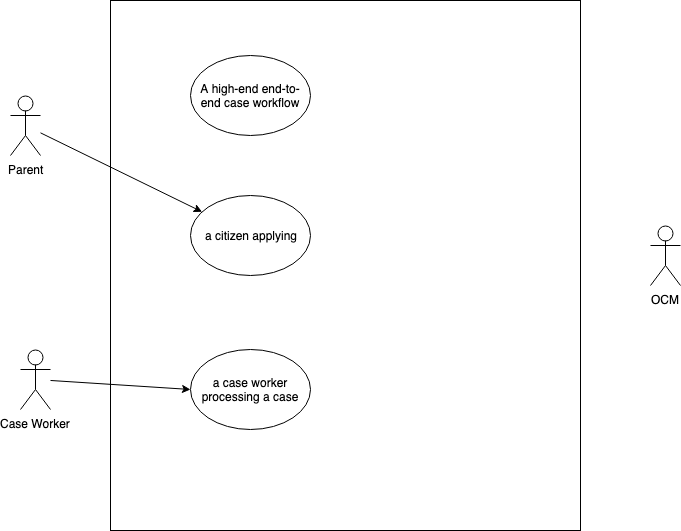
\includegraphics[width=\textwidth]{img/use-cases}
	\caption{Use case diagram}
\end{figure}

\newpage
\section{Detailed Use cases}

\subsection{UC01: A high-end end-to-end case workflow}

\begin{table}[htb!]
\begin{tabularx}{\textwidth}{l|X}
	\textbf{Use Case name} & A high-end end-to-end case workflow \\
	\hline
	\textbf{Participating actor} & Caseworker, User, OCM\\
	\hline
	\textbf{Flow of events} &
	\begin{minipage}{\linewidth}
		\begin{enumerate}
			\item User creates application for loss of earnings,provides all needed information.
			\item Caseworker receives application, processes it and approves it.
			\item OCM sends email about the the approval of the application
			\item Calculation of compensation will be made by OCM
			\item OCM sets application on done\\
		\end{enumerate} 
	\end{minipage}\\
	\hline
	\textbf{Extensions} & 
	\begin{minipage}{\linewidth}
	    \begin{enumerate}
	        \setcounter{enumi}{1}
	        \item \begin{enumerate}
	            \item Caseworker rejects application
	            \item OCM sends mail of rejection
	        \end{enumerate}
	    \end{enumerate}
	\end{minipage}\\
	\hline
	\textbf{Entry condition} &
	Caseworker is logged in
	\\
	\hline
	\textbf{Exit condition} & 
	\begin{minipage}{\linewidth}
	\begin{enumerate}
	    \item Caseworker is logged out
	\end{enumerate}
	\end{minipage}
	\\
	\hline
	\textbf{Quality requirements} & See non-functional requirements in section \ref{sec:nfr}\\
\end{tabularx}
\end{table}


\subsection{UC02: A citizen applying}

\begin{table}[htb!]
\begin{tabularx}{\textwidth}{l|X}
	\textbf{Use Case name} & A citizen applying \\
	\hline
	\textbf{Participating actor} & User, OCM\\
	\hline
	\textbf{Flow of events} & 
	\begin{minipage}{\linewidth}
	    \begin{enumerate}
	        \item User visits the portal
	        \item User initiates the process for applying loss of earnings
	        \item User fills out all the necessary information needed in the form
	        \item User uploads all required documentation
	        \item User uploads a doctor confirmation
	    \end{enumerate}
	\end{minipage}\\
	\hline
	\textbf{Entry condition} & User is logged in\\
	\hline
	\textbf{Exit condition} & User saves the application and logs out\\
	\hline
	\textbf{Quality requirements} & See non-functional requirements in section \ref{sec:nfr}\\
\end{tabularx}
\end{table}

\subsection{UC03: A case worker processing a case}
\begin{table}[htb!]
\begin{tabularx}{\textwidth}{l|X}
	\textbf{Use Case name} & A case worker processing a case \\
	\hline
	\textbf{Participating actor} & Caseworker, OCM\\
	\hline
	\textbf{Flow of events} & 
	\begin{minipage}{\linewidth}
	    \begin{enumerate}
	        \item Caseworker opens a newly opened application
	        \item Caseworker checks the documentation to be legitimate (including the provided doctor confirmation)
	        \item Caseworker approves application
	        \item OCM calculates 
	    \end{enumerate}
	\end{minipage}\\
	\hline
	\textbf{Entry condition} & Caseworker is logged in\\
	\hline
	\textbf{Exit condition} & \\
	\hline
	\textbf{Quality requirements} & See non-functional requirements in section \ref{sec:nfr}\\
\end{tabularx}
\end{table}

\newpage
\section{Architecture model}

\newpage
\section{Project plan}

\subsection{Team composition/roles}
\textbf{Silvan Adrian}
\begin{itemize}
	\item SCRUM Master %otherwise won't make much sense of having a project team without a scrum master
\end{itemize}
\textbf{Matias Korn}
\begin{itemize}
	\item Developer
\end{itemize}
\textbf{Samuel Korn}
\begin{itemize}
	\item Developer
\end{itemize}
\textbf{Nikolin Prenga}
\begin{itemize}
	\item Developer
\end{itemize}

\subsection{Skill matrice}
%fill up
\begin{table}[htb!]
\begin{tabular}{lllll}
 \textbf{Skill}  & \textbf{Silvan} & \textbf{Matias} & \textbf{Samuel} & \textbf{Nikolin} \\
\hline
Development       &                 &                   &                   &                  \\
Project Management &                 &                   &                   &                  \\
                  &                 &                   &                   &                 
\end{tabular}
\end{table}

\subsection{Work Packages}
% just a graph or actually some coding involved?

\subsection{Schedule}
As the project methodology SCRUM will be used, so after each Sprint there will be  working increment released.


\begin{table}[htb!]
\begin{tabular}{lll}
\textbf{Sprint} & \textbf{Sprint Goal} & \textbf{Date} \\
\hline
1      & Set Up Infrastructure & xx.xx \\
2      & Do more etc.          &            \\
3       &                       &           
\end{tabular}
\end{table}

\subsection{Risks}
\begin{table}[htb!]
\begin{tabularx}{\textwidth}{llllXX}
\textbf{Nr} & \textbf{Description} & \textbf{Probability} & \textbf{Criticality} & \textbf{Prevention}                                                      & \textbf{Measure}                                                                             \\
\hline
R1          & Worker gets sick     & 10\%                 & high                 & Every worker should be able to replace the skill of an other in the team & Split up work not only according to someones skills but also to get them to learn new things \\
            &                      &                      &                      &                                                                          &                                                                                              \\
            &                      &                      &                      &                                                                          &                                                                                             
\end{tabularx}
\end{table}

\end{document}
